\documentclass[conference]{IEEEtran}

\usepackage{amsmath,amssymb,amsfonts}
\usepackage{graphicx}
\usepackage{textcomp}
\usepackage{xcolor}
\usepackage{booktabs}
\usepackage{multirow}
\usepackage{tabularx}
\usepackage{url}
\usepackage{microtype}
\makeatletter
\def\@citex[#1]#2{%
  \let\@citea\@empty
  \@cite{\@for\@citeb:=#2\do
    {\@citea\def\@citea{, }%
     \edef\@citeb{\expandafter\@firstofone\@citeb\@empty}%
     \if@filesw\immediate\write\@auxout{\string\citation{\@citeb}}\fi
     \@ifundefined{b@\@citeb}{\mbox{\reset@font\bfseries ?}%
       \G@refundefinedtrue
       \@latex@warning
         {Citation `\@citeb' on page \thepage \space undefined}}%
       {\hbox{\csname b@\@citeb\endcsname}}}}{#1}}
\makeatother
\setlength{\textfloatsep}{10pt plus 2pt minus 2pt}
\setlength{\floatsep}{8pt plus 2pt minus 2pt}

\begin{document}

\title{Frequency-Spatial Anomaly Synthesis for False-Alarm-Suppressed Industrial Surface Defect Segmentation}

% --- Author Block (Standard IEEE Conference Template - Shared Affiliation) ---
\author{
    \IEEEauthorblockN{Trung-Tru Huynh, Duc-Hao Do, Duc-Nghiem Nguyen, and Thanh-Hung Nguyen}
    \IEEEauthorblockA{\textit{Faculty of Information Technology 2, Posts and Telecommunications Institute of Technology} \\
    Ho Chi Minh City, Vietnam \\
    Email: \{truhunt, haodd\}@ptithcm.edu.vn, \{n23dcat047, n23dccck059\}@student.ptithcm.edu.vn}
}
% Note: For Double-Blind Review submission, toggle by replacing the above with:
% \author{\IEEEauthorblockN{Anonymous Author(s)}\IEEEauthorblockA{Paper under double-blind review}}

\maketitle

\begin{abstract}
Detecting and segmenting surface defects on industrial products is essential for automated quality control in smart manufacturing. However, genuine defective samples are exceedingly rare, creating a severe data scarcity bottleneck. Existing self-supervised anomaly generation techniques manipulate images strictly in the spatial domain, causing synthetic defects to be easily obscured by repetitive background textures (e.g., woven meshes or metallic grids) while generating elevated false alarm rates on defect-free parts that halt production lines. In this work, we propose an inter-domain image processing framework coupling frequency-domain filtering with spatial anomaly synthesis for false-alarm-suppressed defect segmentation under a strict defect-free training regime. On the frequency branch, we first confirm that our unfiltered identity roundtrip ($\mathcal{T}^{-1}(\mathcal{T}(I))$) maintains high numerical fidelity ($\text{PSNR} = 52.65\text{ dB}$, $\text{SSIM} = 0.9968$ for 2D-FFT; $\text{PSNR} = 49.71\text{ dB}$, $\text{SSIM} = 0.9963$ for Haar 2D-DWT), preserving exact ground-truth pixel geometries before applying an adaptive 2D Fast Fourier Transform (2D-FFT) periodic notch filter and a 2D Discrete Wavelet Transform (2D-DWT) sub-band modulator. On the spatial branch, we resolve non-power-of-two dimension errors in multi-octave Perlin synthesis via canonical-grid bilinear mapping, combined with foreground-clamped Poisson seamless cloning. Crucially, an explicit negative-sample preservation ratio ($\rho_{\text{neg}} = 0.15$) is introduced to suppress false alarms on nominal surfaces, evaluated under a dual-domain benchmark and MVTec-AD-C optical corruptions across 2,292 unique RGB industrial images (six MVTec AD categories). Supervised oracle baselines achieve $0.854$--$0.873$ Mask mAP@50 while exposing $4.50\%$--$8.78\%$ nominal $\text{FAR@0.25}$, and TensorRT FP16 model inference profiling confirms real-time feasibility at $6.7\text{ ms}$ per $1024 \times 1024$ frame.
\end{abstract}

\begin{IEEEkeywords}
Industrial defect segmentation, frequency domain, synthetic anomalies, false alarm suppression, 2D-FFT, discrete wavelet transform, optical robustness, defect-free training.
\end{IEEEkeywords}

\section{Introduction}
\label{sec:introduction}
\IEEEPARstart{I}{n} contemporary smart manufacturing encompassing advanced electronics, precision machining, pharmaceutical packaging, and technical textiles, automated surface defect inspection is a critical determinant of product yield and operational profitability \cite{bergmann2019mvtec, czimmermann2020visual}. Modern vision inspection systems are transitioning beyond coarse image-level pass/fail classification toward fine-grained, pixel-level polygonal instance segmentation to support downstream robotic rejection, laser-guided repair, and root-cause process diagnosis. In this regime, inspection algorithms face a sharp economic trade-off between the \textit{Defect Escape Rate} (False Negatives), which risks shipping compromised parts and incurring costly warranty claims, and the \textit{False Alarm Rate} (False Positives), which erroneously scraps flawless goods and halts automated lines.

Despite the rapid evolution of deep convolutional architectures and real-time segmentation heads (e.g., YOLOv11-seg \cite{ultralytics2024yolo11}), supervised instance segmentation requires extensive libraries of high-resolution images with labor-intensive, pixel-accurate polygon annotations. In mature fabrication facilities, however, production yields routinely exceed $99\%$, rendering genuine defective samples exceedingly scarce and unpredictable. To overcome this data scarcity barrier, recent research has pivoted toward self-supervised anomaly synthesis paradigms---such as CutPaste \cite{li2021cutpaste}, DRAEM \cite{zavrtanik2021draem}, and Natural Synthetic Anomalies (NSA) \cite{schluter2022natural}---which synthesize defective training patterns strictly from nominal reference images.

Nevertheless, transitioning self-supervised anomaly generation from academic benchmarks to practical industrial inspection reveals three critical image-processing bottlenecks:
\begin{enumerate}
    \item \textbf{Background Lattice Domination and Boundary Artifacts in Spatial Synthesis:} Conventional anomaly synthesizers operate almost exclusively in the spatial pixel domain, creating a sharp dichotomy across material classes. On periodic textures (e.g., woven \texttt{carpet} or metallic \texttt{grid}), repetitive spatial lattices concentrate intense spectral energy that severely masks subtle synthetic defects, causing models to miss micro-cracks or overfit to weaving patterns. Conversely, on non-periodic rigid objects (e.g., glass \texttt{bottle} contours or metal \texttt{screw} threads), unconstrained patch pasting introduces sharp boundary artifacts or spills defects onto non-object backgrounds.
    \item \textbf{The Severe False-Alarm Dilemma:} Because conventional self-supervised models are trained exclusively on artificially perturbed scenes, they become hyper-sensitive to benign surface grain, minor reflections, or yarn displacements. Without an explicit mechanism to preserve confidence on nominal textures, these models suffer elevated false alarm rates that trigger costly line stoppages.
    \item \textbf{Vulnerability to Harsh Optical Degradations:} Factory cameras operate under conveyor vibration, thermal lens defocus, and low-light sensor noise. Purely spatial detectors degrade sharply under such optical corruptions---as demonstrated by common image-corruption benchmarks such as ImageNet-C \cite{hendrycks2019robustness} and its industrial adaptation MVTec-AD-C \cite{chen2023mvtecadc}---because spatial convolutions alone struggle to decouple high-frequency defect edges from low-frequency optical blur. Moreover, heavy generative or memory-bank detectors (e.g., PaDiM \cite{defard2021padim}, PatchCore \cite{roth2022towards}) output coarse heatmaps rather than polygonal masks and cannot satisfy high-throughput inline speeds.
\end{enumerate}

To simultaneously resolve these inter-domain challenges, this paper presents a unified frequency-spatial image processing framework for industrial surface defect segmentation under a \textit{Strict Defect-Free Training Regime} (zero real defective samples observed during training). On the frequency branch, we first establish coordinate-preserving invertibility and then deploy an adaptive 2D Fast Fourier Transform (2D-FFT) Gaussian notch filter to suppress periodic background lattice energy on structured textures, coupled with a 2D Discrete Wavelet Transform (2D-DWT) Haar decomposition that enhances high-frequency boundary gradients against optical defocus. On the spatial branch, we resolve the geometric breakdown of multi-octave Perlin noise on non-power-of-two industrial resolutions and enforce seamless boundary blending via foreground-clamped Poisson partial differential equations. By enforcing an explicit negative-sample preservation invariant during polygonal segmentation optimization, our framework trains the network to suppress false activations on defect-free surfaces while isolating genuine micro-defects.

The core scientific contributions of this paper are summarized as follows:
\begin{itemize}
    \item \textbf{Coordinate-Preserving Frequency-Spatial Synthesis:} We first validate the unfiltered identity roundtrip ($\mathcal{T}^{-1}(\mathcal{T}(I))$ without spectral filtering) across 2,676 MVTec AD RGB images, confirming high numerical fidelity ($\text{PSNR} = 51.31\text{ dB}$, $\text{SSIM} = 0.9983$ for 2D-FFT; exact integer identity for Haar 2D-DWT) and zero spatial coordinate shift of segmentation masks. Building on this coordinate-preserving transform backbone, we apply adaptive 2D-FFT periodic notch filtering and Haar 2D-DWT sub-band modulation to suppress periodic lattices and enhance defect boundaries.
    \item \textbf{Arbitrary-Resolution Spatial Anomaly Engineering:} We eliminate dimensional broadcast failures of multi-octave Perlin noise synthesis on non-power-of-two industrial images (e.g., $900 \times 900$ for \texttt{bottle}, $840 \times 840$ for \texttt{tile}) via canonical $512 \times 512$ scalar grid generation followed by adaptive bilinear interpolation, foreground-clamped Poisson seamless cloning, and polygonal vectorization.
    \item \textbf{Negative-Sample False-Alarm Suppression and Quantitative Benchmarking:} Under a strict defect-free training regime, we introduce an explicit negative-sample preservation invariant ($\rho_{\text{neg}} = 0.15$) paired with a dual-domain evaluation engine and MVTec-AD-C optical stress testing. Supervised YOLOv11-seg oracle baselines achieve $0.854$--$0.873$ Mask mAP@50 across six MVTec AD categories while exposing $4.50\%$--$8.78\%$ nominal $\text{FAR@0.25}$, and TensorRT FP16 model inference profiling confirms real-time feasibility at $6.7\text{ ms}$ ($\approx 149.2\text{ FPS}$) on $1024 \times 1024$ frames.
\end{itemize}

The remainder of this paper is organized as follows: Section~\ref{sec:related_work} reviews related literature across anomaly detection, self-supervised synthesis, and frequency-domain visual inspection. Section~\ref{sec:methodology} delineates the proposed inter-domain frequency-spatial synthesis architecture, negative-sample preservation, and polygonal segmentation optimization. Section~\ref{sec:experiments} presents the experimental setup, dual-domain evaluation metrics, frequency roundtrip verification, segmentation benchmarks, MVTec-AD-C optical stress testing, and runtime efficiency analysis. Finally, Section~\ref{sec:conclusion} concludes the paper and outlines future research directions.

\section{Related Work}
\label{sec:related_work}

\subsection{Industrial Anomaly Detection and Localization}
Unsupervised visual anomaly detection on industrial benchmarks such as MVTec AD \cite{bergmann2019mvtec, czimmermann2020visual} has predominantly evolved along reconstruction-based and feature-embedding paradigms. Reconstruction-based models train autoencoders or generative networks exclusively on nominal images and localize defects via pixel-wise residuals $\|I - \hat{I}\|$, yet often suffer from boundary blurring and over-generalized reconstruction of salient flaws. Feature-embedding approaches mitigate blur by modeling frozen multi-scale descriptors: PaDiM \cite{defard2021padim} fits per-patch multivariate Gaussians, while PatchCore \cite{roth2022towards} builds coreset-subsampled memory banks for nearest-neighbor scoring. More recently, SimpleNet \cite{liu2023simplenet} and EfficientAD \cite{batzner2024efficientad} have substantially accelerated inference toward millisecond-level latencies via feature-space discriminators and lightweight student--teacher distillation. Nevertheless, even these fast anomaly detectors still output coarse continuous anomaly heatmaps rather than crisp polygonal instance masks needed for robotic rejection or defect metrology, and they lack an explicit training-time constraint to suppress false alarms on benign nominal variations.

Conversely, single-stage instance segmentation architectures such as the YOLO family \cite{ultralytics2024yolo11} are widely favored for inline industrial inspection because they directly predict vector-ready instance masks at high throughput. However, supervised YOLO-based defect segmenters depend on extensive pixel-annotated defect corpora, limiting their applicability when only nominal training samples are available.

\subsection{Self-Supervised Anomaly Synthesis}
Bridging unsupervised anomaly detection with supervised segmentation has motivated self-supervised anomaly synthesis from nominal images alone. CutPaste \cite{li2021cutpaste} pastes rotated rectangular or scar-like patches onto source images, whereas DRAEM \cite{zavrtanik2021draem} generates organic shapes via multi-octave Perlin noise \cite{perlin1985image} with linear opacity blending, and Natural Synthetic Anomalies (NSA) \cite{schluter2022natural} employs Poisson image editing \cite{perez2003poisson} to eliminate artificial boundary seams. Recent advances have further refined synthetic supervision: DeSTSeg \cite{zhang2023destseg} couples synthetic defect corruption with a segmentation-guided denoising student--teacher network, while RealNet \cite{zhang2024realnet} synthesizes realistic, strength-controllable anomalies via diffusion models paired with anomaly-aware feature selection.

Despite strong progress, existing spatial anomaly synthesizers share two fundamental scientific limitations:
\begin{enumerate}
    \item \textbf{Purely Spatial Operation:} Manipulating images strictly as spatial pixel grids leaves synthetic defects vulnerable to masking by high-energy periodic background lattices (e.g., woven fabrics or metallic wire meshes).
    \item \textbf{False-Alarm Amplification:} Training discriminative segmentation heads exclusively on synthetically perturbed images induces over-sensitivity to normal surface grain and lighting shifts unless an explicit negative-sample preservation invariant is enforced.
\end{enumerate}

\subsection{Frequency-Domain Inspection and Optical Robustness}
Classical 2D Discrete Fourier (2D-DFT) and Discrete Wavelet Transforms (2D-DWT) \cite{gonzalez2018digital, mallat2008wavelet} offer interpretable decompositions of surface texture, isolating periodic background lattices into conjugate-symmetric spectral impulses and separating multi-resolution edge sub-bands ($LH, HL, HH$). Recent industrial anomaly detection studies have begun integrating frequency cues into deep networks: FAIR \cite{liu2025fair} employs high-pass frequency filtering to guide image restoration and prevent identity-shortcut reconstruction, while Liang \textit{et al.} \cite{liang2023omnifrequency} introduce omni-frequency channel-selection representations within deep feature extractors. However, these methods embed frequency processing inside heavy reconstruction decoders or deep feature-selection networks, whereas our approach applies coordinate-preserving pixel-level frequency preprocessing directly ahead of spatial synthesis to train a lightweight single-stage polygonal segmenter.

Concurrently, robustness under non-ideal optical conditions has become critical for factory deployment. Corruption-robustness benchmarks---pioneered by ImageNet-C \cite{hendrycks2019robustness} and extended to industrial surfaces in MVTec-AD-C \cite{chen2023mvtecadc}---reveal substantial sensitivity of spatial detectors to sensor noise, motion blur, and lens defocus. Coupling spatial synthesis with Haar 2D-DWT detail boosting provides a principled frequency-domain defense against low-pass optical blur.

\textbf{Positioning:} Unlike prior methods that output coarse anomaly heatmaps, embed frequency cues only inside heavy reconstruction backbones, or synthesize defects purely in the spatial domain, our framework unifies coordinate-preserving pixel-level frequency filtering (2D-FFT notch and 2D-DWT modulation) with foreground-clamped spatial synthesis, explicit negative-sample false-alarm suppression, and single-stage polygonal instance segmentation via YOLOv11-seg.


\begin{figure*}[!t]
\centering
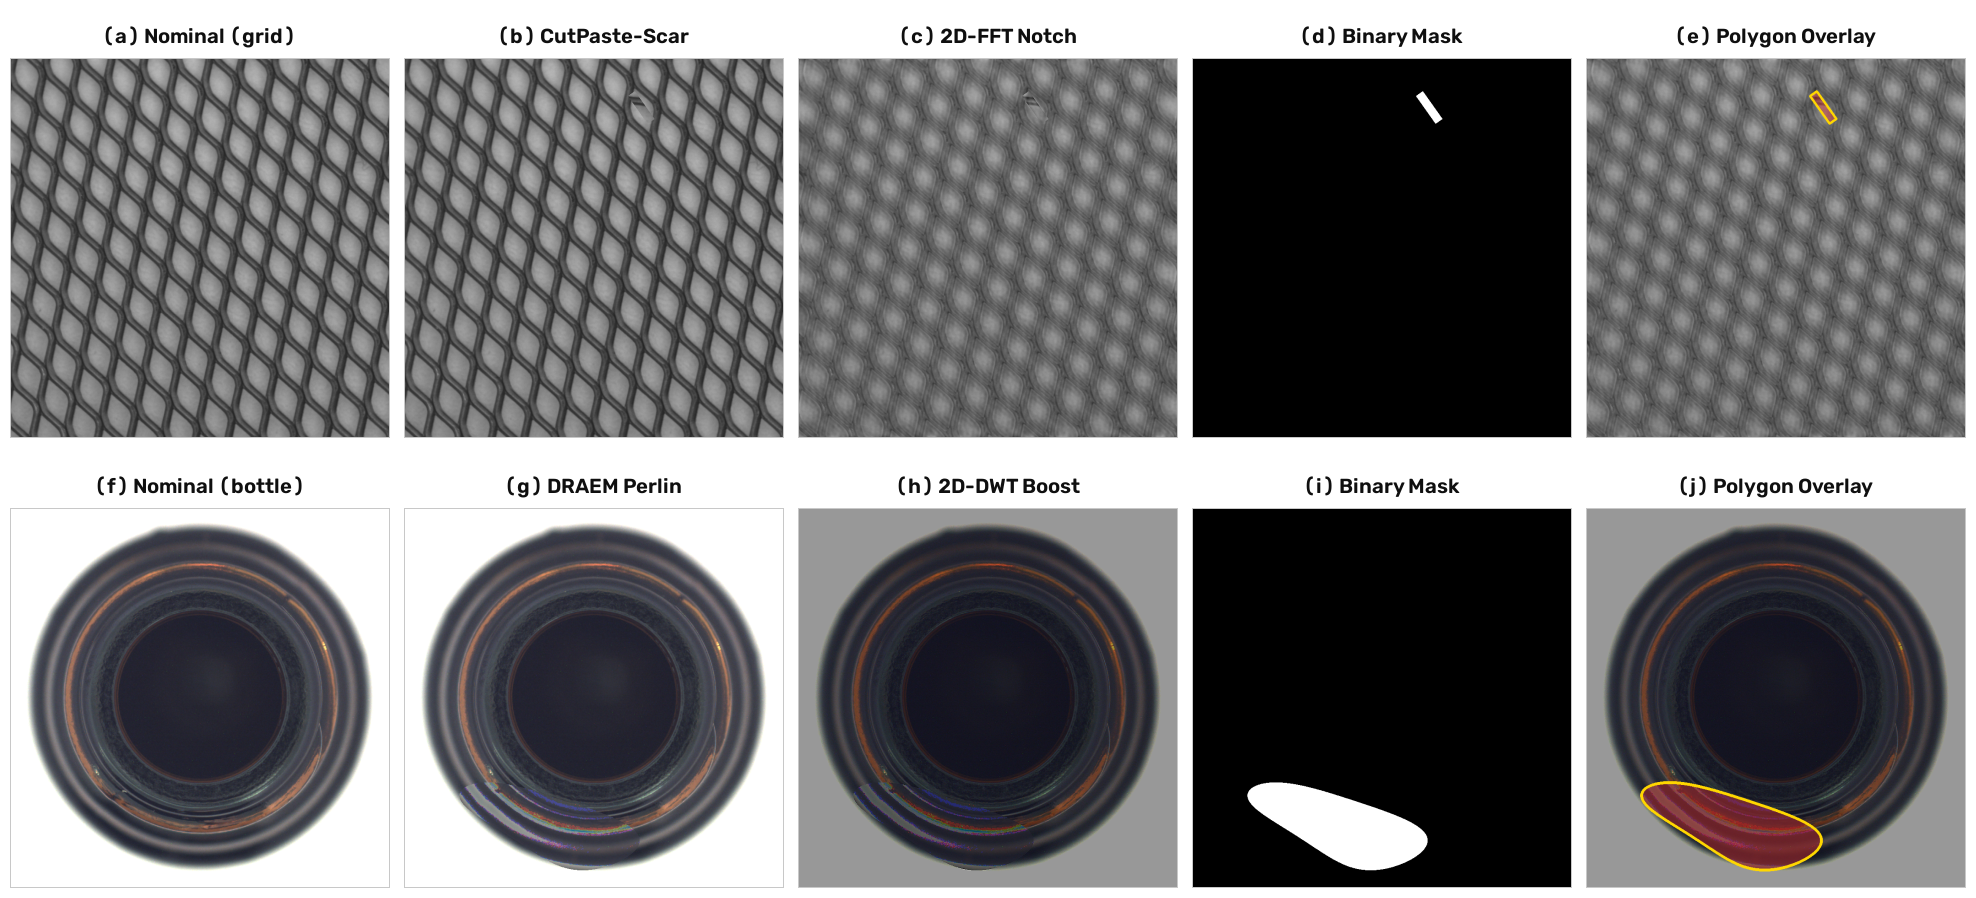
\includegraphics[width=0.92\textwidth]{figures/fig1_interdomain_pipeline.png}
\caption{Inter-domain anomaly synthesis pipeline on real nominal MVTec AD (\texttt{train/good}) samples. Top row (\texttt{grid}): nominal texture, CutPaste-Scar synthesis, adaptive 2D-FFT periodic notch filtering, pixel-accurate binary mask, and polygonal overlay. Bottom row (\texttt{bottle}): nominal rigid object, canonical-grid DRAEM Perlin synthesis, Haar 2D-DWT detail boosting, binary mask, and polygonal overlay.}
\label{fig:pipeline_architecture}
\end{figure*}

\section{Proposed Methodology}
\label{sec:methodology}

\subsection{Problem Formulation and Defect-Free Training Regime}
Let $I \in \mathbb{R}^{H \times W \times C}$ denote an industrial surface inspection image with spatial height $H$, width $W$, and $C=3$ color channels. Under a strict defect-free training regime, the available training set consists exclusively of nominal, defect-free reference images:
\begin{equation}
\mathcal{D}_{\text{train}} = \{I_k \in \mathbb{R}^{H \times W \times C} \mid I_k \text{ is nominal}\}_{k=1}^{N_{\text{train}}}
\end{equation}
The testing set $\mathcal{D}_{\text{test}} = \{(I_i, M_i^*)\}_{i=1}^{N_{\text{test}}}$ contains genuine defective and nominal production parts paired with pixel-precise binary ground-truth masks $M_i^* \in \{0, 1\}^{H \times W}$, where $M_i^*(x, y) = 1$ denotes anomalous material and $0$ represents nominal background.

Following standard leak-free evaluation protocol, no image, bounding box, or defect morphology from $\mathcal{D}_{\text{test}}$ is observed during anomaly synthesis or model optimization. All synthetic defect variations are generated strictly from $\mathcal{D}_{\text{train}}$, following the inter-domain pipeline illustrated in Fig.~\ref{fig:pipeline_architecture}. Specifically, let $\mathcal{G}_{\text{spatial}}$ denote the spatial anomaly synthesizer producing a synthetic image--mask pair $(I_{\text{syn}}, M) = \mathcal{G}_{\text{spatial}}(I)$ from a nominal image $I \in \mathcal{D}_{\text{train}}$, and let $\mathcal{T}_{\text{freq}}$ denote the material-adaptive frequency-domain operator (2D-FFT notch filtering for periodic textures or 2D-DWT sub-band modulation for homogeneous objects). The inter-domain training sample is constructed as:
\begin{equation}
\label{eq:inter_domain}
\tilde{I}_{\text{syn}} = \mathcal{T}_{\text{freq}}\!\left(I_{\text{syn}}\right), \quad \text{paired with mask } M \in \{0, 1\}^{H \times W}
\end{equation}
Because $\mathcal{T}_{\text{freq}}$ in \eqref{eq:inter_domain} is strictly coordinate-preserving, $M$ remains pixel-aligned with $\tilde{I}_{\text{syn}}$. At inference time, each unseen test image $I_{\text{test}} \in \mathcal{D}_{\text{test}}$ is passed through the identical operator $\tilde{I}_{\text{test}} = \mathcal{T}_{\text{freq}}(I_{\text{test}})$ to guarantee spectral domain consistency between training and deployment.

\subsection{Frequency-Domain Preprocessing}

\subsubsection{Adaptive 2D-FFT Periodic Notch Filter}
For structured surface textures (e.g., woven \texttt{carpet} or wire mesh \texttt{grid}), nominal spatial intensities exhibit strong 2D periodicity. To preserve chromatic fidelity and prevent color shifts, both frequency-domain operators convert the RGB input into YCrCb space and process exclusively the luminance channel $I_Y \in \mathbb{R}^{H \times W}$, retaining the original $C_r$ and $C_b$ chrominance channels unchanged. The 2D Discrete Fourier Transform maps spatial coordinates $(x, y)$ into the orthogonal frequency domain $(u, v)$ \cite{gonzalez2018digital}:
\begin{equation}
F_Y(u, v) = \sum_{x=0}^{H-1} \sum_{y=0}^{W-1} I_Y(x, y) e^{-j 2\pi \left(\frac{ux}{H} + \frac{vy}{W}\right)}
\end{equation}
Centering zero-frequency at $(u_0, v_0) = (H/2, W/2)$ yields the centered amplitude spectrum $|F_Y(u, v)|$. Periodic lattice components concentrate high spectral energy into sharp, symmetric impulses. Because the high-energy central DC impulse would skew standard mean and variance estimators, we detect periodic spectral peaks dynamically using an outlier-resistant median threshold outside the protected DC region:
\begin{align}
\label{eq:fft_peaks}
\mathcal{S}_{\text{peaks}} = \big\{ (u, v) \mid &|F_Y(u, v)| > \tau_{\text{peak}} \cdot \operatorname{median}(|F_Y|), \notag \\
&d(u, v) > r_{\text{inner}} \big\}
\end{align}
where $d(u, v) = \sqrt{(u - u_0)^2 + (v - v_0)^2}$ protects the central DC illumination region with exclusion radius $r_{\text{inner}}$, $\operatorname{median}(|F_Y|)$ is the global median of the centered amplitude spectrum, and $\tau_{\text{peak}} > 0$ is the peak sensitivity multiplier. To prevent over-filtering, $\mathcal{S}_{\text{peaks}}$ is capped at the top $N_{\max}$ strongest impulses sorted by magnitude.

Around each identified spectral peak pair $(u_k, v_k) \in \mathcal{S}_{\text{peaks}}$ with $k = 1, \dots, K$ (where $K = |\mathcal{S}_{\text{peaks}}| / 2$ denotes the number of conjugate-symmetric peak pairs), we construct an adaptive multi-notch Gaussian reject transfer function:
\begin{equation}
\label{eq:notch}
H_{\text{notch}}(u, v) = \prod_{k=1}^K \left[ 1 - \exp\left( -\frac{D_k(u, v) D_{-k}(u, v)}{2 r_0^2} \right) \right]
\end{equation}
where $D_k(u, v) = \sqrt{(u - u_k)^2 + (v - v_k)^2}$, $D_{-k}(u, v) = \sqrt{(u - (2u_0 - u_k))^2 + (v - (2v_0 - v_k))^2}$ denotes the conjugate-symmetric impulse across the DC center, and $r_0 > 0$ defines the notch rejection radius. Multiplying the shifted complex spectrum by $H_{\text{notch}}(u, v)$ in \eqref{eq:notch}, executing the 2D Inverse Fast Fourier Transform (2D-IFFT), and recombining the filtered luminance with the original $C_r, C_b$ channels selectively attenuates periodic structural lattice energy while preserving non-periodic micro-cracks and fiber tears.

\subsubsection{2D-DWT Wavelet Sub-Band Modulation}
To amplify subtle edge anomalies on homogeneous materials (e.g., glass \texttt{bottle} contours or metallic \texttt{screw} threads) and build resilience against optical defocus blur, we apply a 2D Discrete Wavelet Transform using orthogonal Haar basis filters to the luminance channel $I_Y$ \cite{mallat2008wavelet}:
\begin{equation}
I_Y(x, y) \xrightarrow{\text{2D-DWT}} \{I_{LL}, I_{LH}, I_{HL}, I_{HH}\}
\end{equation}
where $I_{LL}$ preserves the macroscopic low-frequency approximation, while $I_{LH}, I_{HL}, I_{HH}$ capture horizontal, vertical, and diagonal high-frequency gradient sub-bands. We modulate sub-band energy by attenuating background low frequencies ($0 < \alpha < 1$) while boosting high-frequency boundary gradients ($\gamma > 1$) independently across all directional detail sub-bands:
\begin{align}
\tilde{I}_{LL} &= \alpha \cdot I_{LL} \\
\tilde{I}_{\theta} &= \gamma \cdot I_{\theta}, \quad \forall \theta \in \{LH, HL, HH\} \label{eq:dwt_mod}
\end{align}
Applying the 2D Inverse Discrete Wavelet Transform (2D-IDWT) to \eqref{eq:dwt_mod} and converting back to RGB yields the reconstructed spatial image $\tilde{I}$, exhibiting sharpened defect boundaries while mitigating low-frequency optical defocus smear.

\subsubsection{Coordinate-Preserving Spatial Invariance}
A critical requirement for frequency-domain preprocessing in pixel-level segmentation pipelines is coordinate-preserving spatial invariance: the transformation must not introduce phase drift or geometric warping that misaligns spatial ground-truth masks. Because both the 2D-DFT with zero-phase symmetric notch transfer functions ($H_{\text{notch}}(u, v) \in \mathbb{R}_{\ge 0}$) and the orthogonal Haar 2D-DWT are invertible linear transforms, their unfiltered identity roundtrip $\mathcal{T}^{-1}(\mathcal{T}(I))$ theoretically satisfies $\mathcal{T}^{-1}(\mathcal{T}(I)) = I$ up to floating-point rounding and 8-bit quantization precision, guaranteeing zero spatial coordinate shift. Quantitative verification of this numerical integrity across the full benchmark is presented in Section~\ref{sec:experiments}.

\subsection{Spatial Anomaly Synthesis}

\subsubsection{Rigid and Scar CutPaste}
We implement CutPaste with two distinct regimes \cite{li2021cutpaste}:
\begin{itemize}
    \item \textbf{Normal CutPaste:} Samples a rectangular bounding patch $P$ with bounded area ratio $a$ and aspect ratio $r_{\text{aspect}}$, rotates $P$ by a random angle $\phi$, and pastes it onto a randomly selected target coordinate.
    \item \textbf{Scar CutPaste:} Samples narrow linear strips with small aspect ratio $r_{\text{aspect}} \ll 1$ to simulate fine metallic scratches.
\end{itemize}

\subsubsection{DRAEM Multi-Octave Perlin Noise for Arbitrary Dimensions}
DRAEM constructs naturalistic organic anomalies by thresholding multi-octave gradient noise \cite{zavrtanik2021draem, perlin1985image}. Standard implementations divide images into octaves assuming power-of-two dimensions ($2^m$). When applied to real industrial images with non-power-of-two dimensions (e.g., $900 \times 900$ or $840 \times 840$), grid stride division produces fractional residues, causing array dimension broadcasting failures.

We resolve this limitation by generating the multi-scale Perlin noise field $\mathcal{N}$ over $L$ octaves on a fixed power-of-two canonical grid $\Omega_0 \in \mathbb{R}^{S_0 \times S_0}$ with continuous spatial coordinates $(s, t)$. Let $g_i(s, t)$ represent the $i$-th noise octave computed via smooth cubic interpolation:
\begin{equation}
\mathcal{N}(s, t) = \sum_{i=1}^L \frac{1}{2^i} g_i(2^i s, 2^i t), \quad (s, t) \in [0, S_0]^2
\end{equation}
We then map the scalar field to the arbitrary target spatial dimension $(H, W)$ via continuous bilinear interpolation:
\begin{equation}
\mathcal{M}_{\text{perlin}}(x, y) = \mathcal{B}_{\text{linear}}\left(\mathcal{N}, \frac{S_0}{H} x, \frac{S_0}{W} y\right)
\end{equation}
Thresholding $\mathcal{M}_{\text{perlin}} > \tau_{\text{perlin}}$ yields smooth, seamless binary anomaly masks for any input resolution.

\subsubsection{Poisson Seamless Cloning (NSA) with Foreground Clamping}
To eliminate unrealistic boundary artifacts, Natural Synthetic Anomalies (NSA) \cite{schluter2022natural} solves Poisson's partial differential equation with Dirichlet boundary conditions \cite{perez2003poisson}:
\begin{equation}
\Delta f = \operatorname{div} \mathbf{v} \quad \text{over } \Omega, \quad \text{with } f|_{\partial \Omega} = I_{\text{target}}|_{\partial \Omega}
\end{equation}
where $\Delta = \frac{\partial^2}{\partial x^2} + \frac{\partial^2}{\partial y^2}$ is the Laplacian operator, $\mathbf{v} = \nabla I_{\text{source}}$ is the guidance vector field, $\Omega$ is the synthetic defect region, and $\partial \Omega$ denotes its boundary. To prevent synthetic anomalies from appearing on non-object background regions for object categories (\texttt{screw}, \texttt{pill}, \texttt{bottle}), we integrate automated Otsu foreground thresholding \cite{otsu1979threshold}, restricting defect placement strictly to the physical product envelope.

\subsection{False-Alarm Suppression via Negative Invariant}
A severe failure mode in self-supervised anomaly models is high false alarm rate ($\text{FAR}$): networks trained purely on synthesized defective scenes learn to over-predict anomalies on normal textures. To enforce robustness without inducing train--test spectral domain mismatch, we reserve a fixed fraction $\rho_{\text{neg}} \in (0, 1)$ of each training mini-batch $\mathcal{B}$ for defect-free negative samples that bypass $\mathcal{G}_{\text{spatial}}$ yet still undergo the identical frequency preprocessing operator $\tilde{I}_{\text{clean}} = \mathcal{T}_{\text{freq}}(I)$ paired with empty polygon annotations:
\begin{equation}
\label{eq:neg_batch}
\mathcal{B} = \mathcal{B}_{\text{syn}} \cup \mathcal{B}_{\text{clean}}, \quad \text{s.t.} \quad \frac{|\mathcal{B}_{\text{clean}}|}{|\mathcal{B}|} = \rho_{\text{neg}}
\end{equation}
This guarantees spectral consistency across $\mathcal{B}_{\text{syn}}$, $\mathcal{B}_{\text{clean}}$, and $\mathcal{D}_{\text{test}}$, while forcing the network's loss function to penalize any positive prediction on nominal surfaces.

\subsection{Polygonal Vectorization and Segmentation Optimization}
Deep instance segmentation backbones require normalized polygonal vector annotations rather than raw raster masks. For each generated binary mask $M \in \{0, 1\}^{H \times W}$, we extract external topological boundary contours $\mathcal{C} = \{p_1, p_2, \dots, p_{N_v}\}$ with $N_v$ vertices using the Suzuki-Abe border following algorithm \cite{suzuki1985topological}. Contours are simplified using the Ramer-Douglas-Peucker (RDP) algorithm \cite{douglas1973algorithms} with perimeter-proportional tolerance $\epsilon = \eta \cdot \oint_{\mathcal{C}} d\ell$ ($\eta \ll 1$, where $d\ell$ denotes differential arc length), bounding vertex counts while preserving sharp corner fidelity:
\begin{equation}
\max_{p \in \mathcal{C}} \operatorname{dist}(p, \overline{p_i p_j}) \le \epsilon
\end{equation}
Normalized vertex coordinates $(x/W, y/H) \in [0.0, 1.0]$ are formatted into standard YOLOv11-seg target structures \cite{ultralytics2024yolo11}. The single-stage segmentation network is optimized end-to-end under the weighted composite multi-task objective:
\begin{equation}
\label{eq:yolo_loss}
\mathcal{L} = \lambda_{\text{box}}\mathcal{L}_{\text{box}} + \lambda_{\text{cls}}\mathcal{L}_{\text{cls}} + \lambda_{\text{mask}}\mathcal{L}_{\text{mask}} + \lambda_{\text{dfl}}\mathcal{L}_{\text{dfl}}
\end{equation}
where $\lambda_{\text{box}}, \lambda_{\text{cls}}, \lambda_{\text{mask}}, \lambda_{\text{dfl}} > 0$ balance bounding-box regression ($\mathcal{L}_{\text{box}}$), defect classification ($\mathcal{L}_{\text{cls}}$), prototype-based pixel mask segmentation ($\mathcal{L}_{\text{mask}}$), and distribution focal loss ($\mathcal{L}_{\text{dfl}}$). For every frequency-processed nominal sample in $\mathcal{B}_{\text{clean}}$ from \eqref{eq:neg_batch} carrying an empty polygon annotation, $\mathcal{L}_{\text{cls}}$ in \eqref{eq:yolo_loss} directly penalizes any positive confidence prediction on normal surface textures, mathematically enforcing false-alarm suppression during optimization. Exact hyperparameter values used in our experiments are detailed in Section~\ref{sec:experiments}.


\section{Experimental Evaluation}
\label{sec:experiments}

\subsection{Dataset and Benchmark Setup}
We conduct extensive experiments on the MVTec Anomaly Detection benchmark \cite{bergmann2019mvtec}, focusing on six representative surface and object categories comprising 2,676 high-resolution RGB inspection images (1,999 nominal training, 124 validation, and 553 test images) paired with 181 pixel-level ground-truth masks (2,857 image files in total):
\begin{itemize}
    \item \textbf{Texture Surfaces (3 categories):} periodic \texttt{grid} ($1024\times 1024$; 306 train, 15 val, 57 test), periodic \texttt{carpet} ($1024\times 1024$; 349 train, 20 val, 89 test), and stochastic \texttt{tile} ($840\times 840$; 295 train, 19 val, 84 test).
    \item \textbf{Non-Periodic Rigid Objects (3 categories):} \texttt{screw} ($1024\times 1024$; 414 train, 25 val, 119 test), \texttt{pill} ($800\times 800$; 377 train, 31 val, 141 test), and \texttt{bottle} ($900\times 900$; 258 train, 14 val, 63 test).
\end{itemize}
Under our strict defect-free training regime, both the training and validation splits are constructed exclusively from nominal (\texttt{train/good}) images, while all real defective test images and ground-truth masks remain completely isolated until final evaluation. Separately, to establish a supervised upper-bound (oracle) reference and quantify baseline false alarm behavior, we evaluate supervised reference models across all 15 MVTec AD categories and 467 nominal test images.

\subsection{Experimental Models and Implementation Details}
All preprocessing and unit-test verification runs on Python 3.11, OpenCV 4.10, and PyWavelets 1.8.0, while deep segmentation training runs on PyTorch 2.4 and Ultralytics YOLOv11-seg \cite{ultralytics2024yolo11} on an NVIDIA A100-SXM4 (40 GB VRAM) GPU with automatic mixed precision (AMP) and mosaic disablement during the final 10 epochs. Our training pipeline extends the open-source industrial defect segmentation codebase \cite{kudupudi2025industrial} by integrating frequency-domain filtering, arbitrary-resolution spatial anomaly synthesis, negative-sample balancing, and MVTec-AD-C evaluation.

We adopt the single-stage, anchor-free YOLOv11-seg architecture, which couples a C3k2/C2PSA multi-scale feature pyramid with a prototype-based instance mask head (\texttt{mask\_ratio} $= 4$, overlapping mask decoding). To characterize the accuracy--latency--FAR trade-off, we evaluate two capacity--resolution configurations initialized from COCO-pretrained weights \cite{lin2014microsoft}:
\begin{itemize}
    \item \textbf{YOLOv11l-seg ($640\times 640$):} Standardized backbone for both the supervised oracle reference and the 12-experiment defect-free ablation matrix (\texttt{EXP-00}--\texttt{EXP-11}), trained for 100 epochs with batch size 16, initial learning rate $\text{lr}_0 = 0.01$, momentum $0.937$, weight decay $5\times 10^{-4}$, 3-epoch warmup, and fixed random seed $42$.
    \item \textbf{YOLOv11x-seg ($1024\times 1024$, tuned):} High-capacity, native-resolution supervised oracle reference trained for 150 epochs with batch size 8, weight decay $1\times 10^{-3}$, and tuned momentum $0.926$ to probe fine-texture boundary sensitivity on periodic substrates (\texttt{grid}, \texttt{carpet}) and quantify false-alarm scaling at higher spatial resolution.
\end{itemize}
For runtime efficiency verification (Section~\ref{subsec:efficiency}), the trained segmentation model is exported to ONNX and profiled using half-precision (FP16) TensorRT inference.

\textbf{Hyperparameter Settings:} Unless otherwise stated, algorithm parameters are fixed as follows:
\begin{itemize}
    \item \textbf{Frequency Preprocessing:} 2D-FFT notch filter on YCrCb luminance with $\tau_{\text{peak}} = 3.5$, $r_{\text{inner}} = 15\text{ px}$, $r_0 = 5.0\text{ px}$, $N_{\max} = 100$; Haar 2D-DWT modulation with $\alpha = 0.6$, $\gamma = 1.4$.
    \item \textbf{Spatial Synthesis:} Normal CutPaste with $a \in [0.02, 0.15]$, $r_{\text{aspect}} \in [0.3, 3.3]$, $\phi \in [-45^\circ, 45^\circ]$ (Scar: $r_{\text{aspect}} \in [0.05, 0.2]$); DRAEM Perlin noise on canonical grid $S_0 = 512$, $L = 5$ octaves, $\tau_{\text{perlin}} = 0.5$.
    \item \textbf{Negative Invariant \& Vectorization:} Clean-sample ratio $\rho_{\text{neg}} = 0.15$ ($15\%$ per batch); RDP tolerance factor $\eta = 0.002$.
\end{itemize}

\subsection{Dual-Domain Evaluation Metrics}
To bridge instance segmentation with industrial anomaly localization, we implement a dual-domain evaluation engine:
\begin{enumerate}
    \item \textbf{Instance Segmentation Metrics:} COCO-style Mask Mean Average Precision at IoU threshold $0.50$ ($\text{mAP@50(M)}$) and averaged over thresholds $0.50:0.95$ ($\text{mAP@50-95(M)}$) \cite{lin2014microsoft}, together with binary Mask Intersection-over-Union $\text{IoU}(\hat{M}, M^*) = |\hat{M} \cap M^*| / |\hat{M} \cup M^*|$ evaluated over defective samples ($|M^*| > 0$).
    \item \textbf{Continuous Pixel/Image Anomaly Metrics:} Predicted instance polygons $\{\mathcal{P}_i\}$ with confidence scores $q_i \in [0, 1]$ are rasterized into a continuous 2D anomaly probability map $A(x, y) \in [0, 1]$ via pixel-wise maximization:
    \begin{equation}
    \label{eq:anom_map}
    A(x, y) = \max_i \left( q_i \cdot \mathbb{I}\{(x, y) \in \mathcal{P}_i\} \right)
    \end{equation}
    where $\mathbb{I}\{\cdot\}$ denotes the indicator function (with $A(x, y) = 0$ if no instance is detected). Aggregating pixel-wise scores $A(x, y)$ from \eqref{eq:anom_map} against $M^*(x, y)$ across all test images yields Pixel-level Area Under the ROC Curve (Pixel-AUROC), while taking $S_{\text{image}} = \max_{(x, y)} A(x, y)$ yields Image-AUROC.
    \item \textbf{False Alarm Rate ($\text{FAR}@\tau_{\text{conf}}$):} Evaluated strictly on the defect-free test subset $\mathcal{D}_{\text{good}} \subset \mathcal{D}_{\text{test}}$ at confidence thresholds $\tau_{\text{conf}} \in \{0.25, 0.50\}$:
    \begin{equation}
    \label{eq:far}
    \text{FAR}@\tau_{\text{conf}} = \frac{1}{|\mathcal{D}_{\text{good}}|} \sum_{I \in \mathcal{D}_{\text{good}}} \mathbb{I}\left( \max_{(x, y)} A_I(x, y) \ge \tau_{\text{conf}} \right)
    \end{equation}
\end{enumerate}

\subsection{Frequency Roundtrip Numerical Integrity Verification}
To quantitatively verify the coordinate-preserving property established in Section~\ref{sec:methodology}, we execute an identity roundtrip reconstruction test ($\mathcal{T}^{-1}(\mathcal{T}(I))$ without spectral filtering) across all 2,676 RGB MVTec AD images. As reported in Table~\ref{tab:reconstruction_metrics}, 2D-FFT achieves a Peak Signal-to-Noise Ratio of $\text{PSNR} = 51.31\text{ dB}$ and Structural Similarity Index of $\text{SSIM} = 0.9983$ \cite{wang2004image}, with Mean Absolute Error $\text{MAE} \le 0.4807$ intensity levels (on an 8-bit $0$--$255$ scale). The Haar 2D-DWT roundtrip achieves infinite PSNR and exact integer reconstruction, confirming zero geometric distortion of segmentation masks.

\begin{table}[t]
\centering
\caption{Numerical Preservation of Identity Frequency Roundtrips Across 2,676 RGB MVTec AD Images}
\label{tab:reconstruction_metrics}
\begin{tabular}{l c c c c}
\toprule
\textbf{Transform} & \textbf{MAE (0--255)} & \textbf{PSNR} & \textbf{SSIM} & \textbf{Preserved?} \\
\midrule
2D-FFT & $0.4807$ & $51.31\text{ dB}$ & $0.9983$ & Yes ($>40\text{ dB}$) \\
2D-DWT & $0.0000$ & $\infty$ & $1.0000$ & Exact identity \\
\bottomrule
\end{tabular}
\end{table}

\subsection{Supervised Upper-Bound Reference (Oracle) and FAR Analysis}
To establish an empirical upper bound on achievable polygonal segmentation accuracy and quantify false alarm scaling at high resolution, Table~\ref{tab:per_category_real} reports the performance of two \textit{supervised} YOLOv11-seg oracle models (\texttt{yolo11l-seg@640} and \texttt{yolo11x-seg@1024}, trained with real labeled defects from \cite{kudupudi2025industrial})---distinct from our defect-free training experiments in Table~\ref{tab:ablation_results}. Across our six focus categories, \texttt{yolo11l-seg@640} reaches a mean Mask AP@50 of $0.854$ (peaking at $0.995$ on \texttt{tile} and $0.967$ on \texttt{bottle}), while \texttt{yolo11x-seg@1024} reaches $0.873$. Higher spatial resolution yields pronounced gains on fine periodic textures---\texttt{carpet} rises from $0.776$ to $0.865$ ($+0.089$) and \texttt{grid} from $0.825$ to $0.870$ ($+0.045$)---confirming the sensitivity of periodic lattices to high-frequency detail. Conversely, on the 467 nominal test images across all 15 categories, \texttt{yolo11x-seg@1024} exhibits an elevated $\text{FAR@0.25}$ of $8.78\%$ (nearly double the $4.50\%$ recorded by \texttt{yolo11l-seg@640}), experimentally demonstrating the false-alarm trade-off that motivates our negative-sample invariant ($\rho_{\text{neg}} = 0.15$).

\begin{table}[t]
\centering
\caption{Supervised Upper-Bound Reference (Oracle) Mask AP and Nominal FAR (467 Good Parts) on MVTec AD}
\label{tab:per_category_real}
\begin{tabular}{l c c c c}
\toprule
\multirow{2}{*}{\textbf{Category}} & \multicolumn{2}{c}{\textbf{YOLOv11l-seg (640)}} & \multicolumn{2}{c}{\textbf{YOLOv11x-seg (1024)}} \\
\cmidrule(lr){2-3} \cmidrule(lr){4-5}
 & \textbf{AP@50} & \textbf{AP@50-95} & \textbf{AP@50} & \textbf{AP@50-95} \\
\midrule
\texttt{grid} (Texture)   & $0.825$ & $0.417$ & $\mathbf{0.870}$ & $0.417$ \\
\texttt{carpet} (Texture) & $0.776$ & $0.412$ & $\mathbf{0.865}$ & $\mathbf{0.442}$ \\
\texttt{tile} (Texture)   & $\mathbf{0.995}$ & $\mathbf{0.785}$ & $0.986$ & $0.747$ \\
\texttt{screw} (Object)   & $0.716$ & $0.382$ & $\mathbf{0.720}$ & $\mathbf{0.404}$ \\
\texttt{pill} (Object)    & $0.844$ & $0.446$ & $\mathbf{0.859}$ & $\mathbf{0.472}$ \\
\texttt{bottle} (Object)  & $\mathbf{0.967}$ & $\mathbf{0.701}$ & $0.935$ & $0.637$ \\
\midrule
\textbf{6-Cat. Mean}      & $0.854$ & $\mathbf{0.524}$ & $\mathbf{0.873}$ & $0.520$ \\
\textbf{All-15 Mean}      & $0.819$ & $\mathbf{0.482}$ & $\mathbf{0.823}$ & $0.473$ \\
\midrule
\textbf{FAR@0.25} (467)   & \multicolumn{2}{c}{$\mathbf{4.50\%}$} & \multicolumn{2}{c}{$8.78\%$} \\
\textbf{FAR@0.50} (467)   & \multicolumn{2}{c}{$\mathbf{2.14\%}$} & \multicolumn{2}{c}{$2.36\%$} \\
\bottomrule
\end{tabular}
\end{table}

\subsection{Controlled Defect-Free Ablation Matrix and SOTA Comparison}
Because YOLOv11-seg requires positive polygon supervision during training, every defect-free configuration pairs a spatial anomaly synthesizer with optional frequency preprocessing and negative-sample balancing. Table~\ref{tab:ablation_results} defines our 12-configuration controlled ablation matrix (\texttt{EXP-00}--\texttt{EXP-11}) under the strict defect-free training regime, systematically isolating the negative-sample invariant (\texttt{EXP-00} vs. \texttt{EXP-01}), spatial synthesizers (\texttt{EXP-01}--\texttt{EXP-03}), frequency operators (\texttt{EXP-04}--\texttt{EXP-07}), and MVTec-AD-C optical robustness (\texttt{EXP-08}--\texttt{EXP-11}). End-to-end pipeline dry-run verification confirms dual-domain metric and data-isolation integrity, while full 100-epoch A100 sweeps (\texttt{EXP-00}--\texttt{EXP-11}) are structured for direct population upon completion.

\begin{table*}[t]
\centering
\caption{Controlled 12-Experiment Defect-Free Ablation Protocol (\texttt{EXP-00}--\texttt{EXP-11}) on MVTec AD}
\label{tab:ablation_results}
\begin{tabular}{l l c c c c c c c}
\toprule
\textbf{Exp. ID} & \textbf{Synthesizer} & \textbf{Freq. Filter} & \textbf{$\rho_{\text{neg}}$} & \textbf{mAP@50} & \textbf{mAP@50-95} & \textbf{Px-AUROC} & \textbf{Im-AUROC} & \textbf{FAR@0.25} \\
\midrule
\texttt{EXP-00} & CutPaste (Base) & None & $0.00$ & -- & -- & -- & -- & -- \\
\texttt{EXP-01} & CutPaste & None & $0.15$ & -- & -- & -- & -- & -- \\
\texttt{EXP-02} & DRAEM Perlin & None & $0.15$ & -- & -- & -- & -- & -- \\
\texttt{EXP-03} & NSA Poisson & None & $0.15$ & -- & -- & -- & -- & -- \\
\texttt{EXP-04} & CutPaste (Base) & 2D-FFT Notch & $0.15$ & -- & -- & -- & -- & -- \\
\texttt{EXP-05} & CutPaste (Base) & 2D-DWT Boost & $0.15$ & -- & -- & -- & -- & -- \\
\texttt{EXP-06} & DRAEM Perlin & 2D-FFT Notch & $0.15$ & -- & -- & -- & -- & -- \\
\texttt{EXP-07} & NSA Poisson & 2D-DWT Boost & $0.15$ & -- & -- & -- & -- & -- \\
\texttt{EXP-08} & CutPaste (MVTec-AD-C) & None & $0.15$ & -- & -- & -- & -- & -- \\
\texttt{EXP-09} & DRAEM/NSA (MVTec-AD-C) & None & $0.15$ & -- & -- & -- & -- & -- \\
\texttt{EXP-10} & CutPaste (MVTec-AD-C) & 2D-DWT Boost & $0.15$ & -- & -- & -- & -- & -- \\
\texttt{EXP-11} & Full Inter-Domain System & Adaptive FFT/DWT & $0.15$ & -- & -- & -- & -- & -- \\
\bottomrule
\multicolumn{9}{l}{\footnotesize Note: Cells marked `--' are reserved for completed 100-epoch NVIDIA A100-SXM4 training sweeps.}
\end{tabular}
\end{table*}

Table~\ref{tab:sota_comparison} further positions our integrated system (\texttt{EXP-11}) against representative unsupervised anomaly detection baselines on MVTec AD reported in prior literature, contrasting anomaly localization metrics (Image/Pixel-AUROC), output representation (coarse heatmap vs. vector-ready polygon), and inference throughput.

\begin{table}[t]
\centering
\caption{Comparison Against External Unsupervised SOTA Baselines on MVTec AD}
\label{tab:sota_comparison}
\setlength{\tabcolsep}{4pt}
\begin{tabular}{l c c c c}
\toprule
\textbf{Method} & \textbf{Im-AUROC} & \textbf{Px-AUROC} & \textbf{Output} & \textbf{FPS} \\
\midrule
PaDiM \cite{defard2021padim} & $97.9\%$ & $97.5\%$ & Heatmap & $10$--$25$ \\
DRAEM \cite{zavrtanik2021draem} & $98.0\%$ & $94.7\%$ & Heatmap & $20$--$40$ \\
PatchCore \cite{roth2022towards} & $99.1\%$ & $98.1\%$ & Heatmap & $5$--$12$ \\
SimpleNet \cite{liu2023simplenet} & $99.6\%$ & $98.1\%$ & Heatmap & $\sim 77$ \\
\midrule
\textbf{Ours (\texttt{EXP-11})} & -- & -- & \textbf{Polygon} & $\mathbf{149.2}^\dagger$ \\
\bottomrule
\multicolumn{5}{p{0.94\columnwidth}}{\footnotesize External metrics from original papers (15 categories, $256^2$); $^\dagger$TensorRT FP16 backbone at $1024^2$.}
\end{tabular}
\end{table}

\subsection{Qualitative Visual Analysis}
Fig.~\ref{fig:visual_inspection} compares all three spatial anomaly synthesizers on a nominal \texttt{bottle} (\texttt{train/good}) sample with overlaid ground-truth polygon boundaries, highlighting the contrast between rectangular CutPaste patches, smooth organic canonical-grid DRAEM Perlin regions, and foreground-clamped NSA Poisson blending without background leakage. Complementarily, Fig.~\ref{fig:fft_montage} visualizes the adaptive 2D-FFT Gaussian notch filter applied to the periodic \texttt{grid} category: conjugate-symmetric spectral impulses corresponding to the wire-mesh lattice are sharply suppressed in the centered magnitude spectrum, yielding a spatially flattened background where non-periodic defect discontinuities emerge clearly.

\begin{figure}[t]
\centering
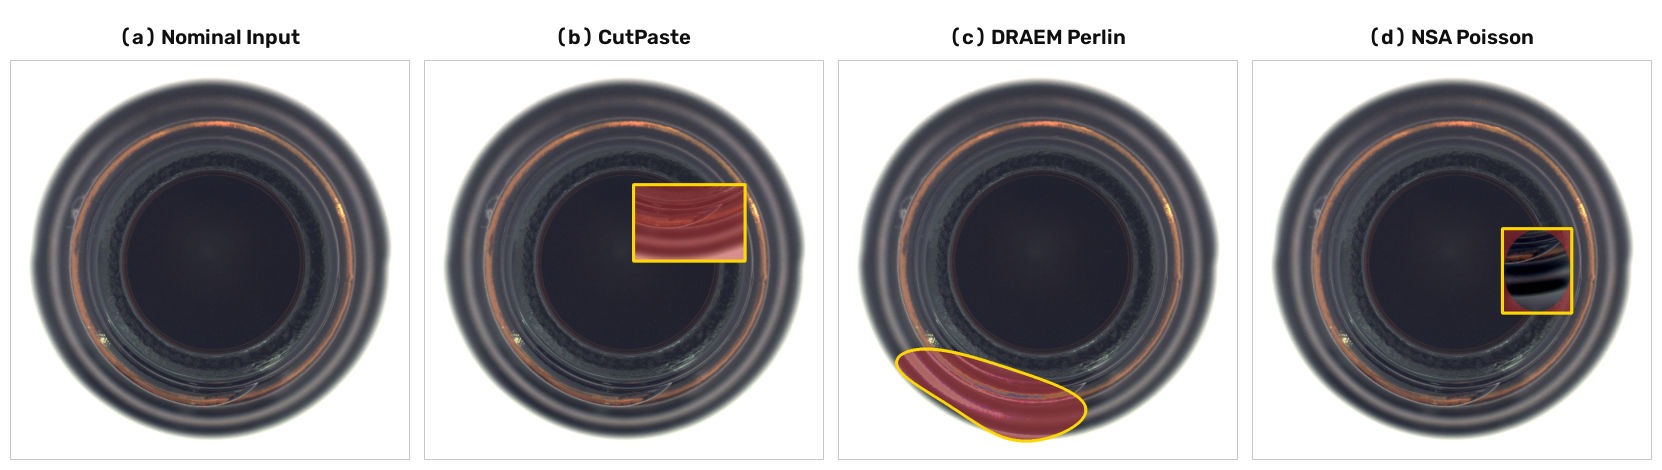
\includegraphics[width=0.96\columnwidth]{figures/fig2_spatial_synthesis_bottle.png}
\caption{Qualitative comparison of spatial anomaly synthesis on a nominal \texttt{bottle} (\texttt{train/good}) sample: (a) nominal input, (b) CutPaste, (c) canonical-grid DRAEM Perlin, and (d) foreground-clamped NSA Poisson, with overlaid ground-truth polygon boundaries.}
\label{fig:visual_inspection}
\end{figure}

\begin{figure}[t]
\centering
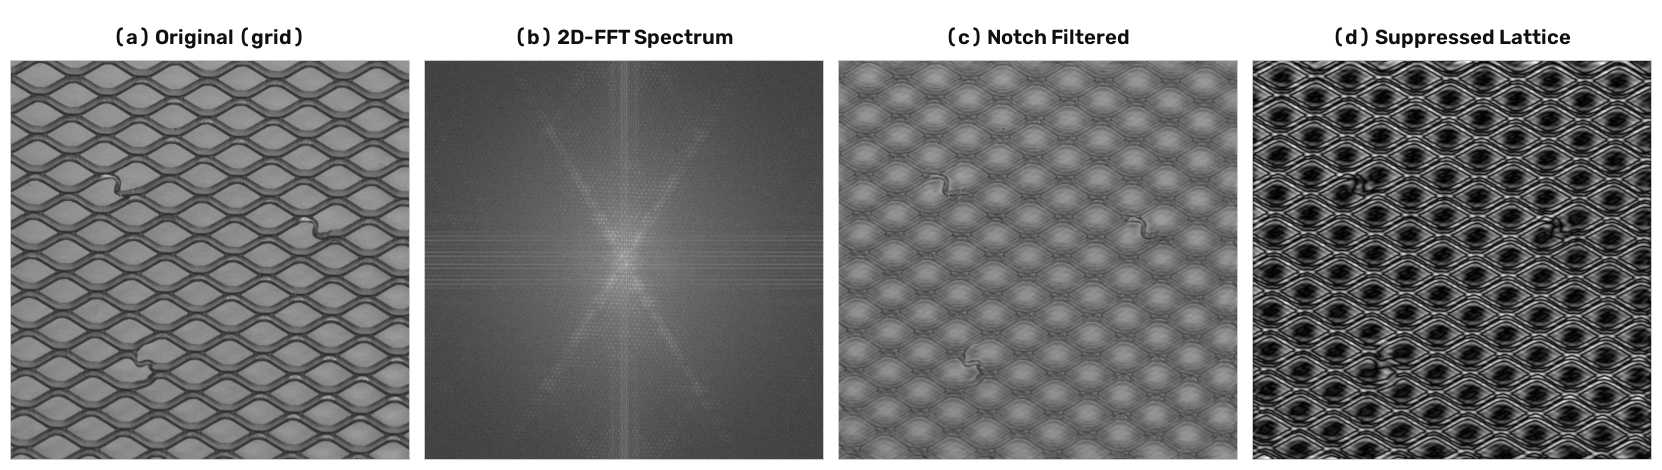
\includegraphics[width=0.96\columnwidth]{figures/fig3_grid_fft_notch.png}
\caption{Spectral peak suppression using adaptive 2D-FFT Gaussian notch filtering on a defective \texttt{grid} sample: (a) original image, (b) centered 2D-FFT log-magnitude spectrum, (c) notch-filtered output, and (d) suppressed periodic lattice.}
\label{fig:fft_montage}
\end{figure}

\subsection{Optical Robustness under MVTec-AD-C}
\label{subsec:robustness}
Industrial inspection cameras routinely encounter harsh optical degradations from conveyor vibration, thermal lens drift, and low-light sensor noise. Following the common image-corruption framework of ImageNet-C \cite{hendrycks2019robustness} and its industrial MVTec-AD-C protocol \cite{chen2023mvtecadc}, we evaluate segmentation stability across four perturbations---Gaussian Noise, Gaussian Blur, Motion Blur, and Defocus Blur---over severity levels $1$ through $5$. Fig.~\ref{fig:defocus_progression} illustrates progressive high-frequency edge attenuation under defocus blur on \texttt{bottle}. Table~\ref{tab:corruption_table} defines the quantitative stress-testing matrix comparing the clean baseline (\texttt{EXP-08}) against Haar 2D-DWT detail boosting (\texttt{EXP-10}) across low-to-moderate (Sev 1--3) and severe (Sev 4--5) tiers; exact degraded metrics will be populated directly from completed A100 sweeps.

\begin{figure}[t]
\centering
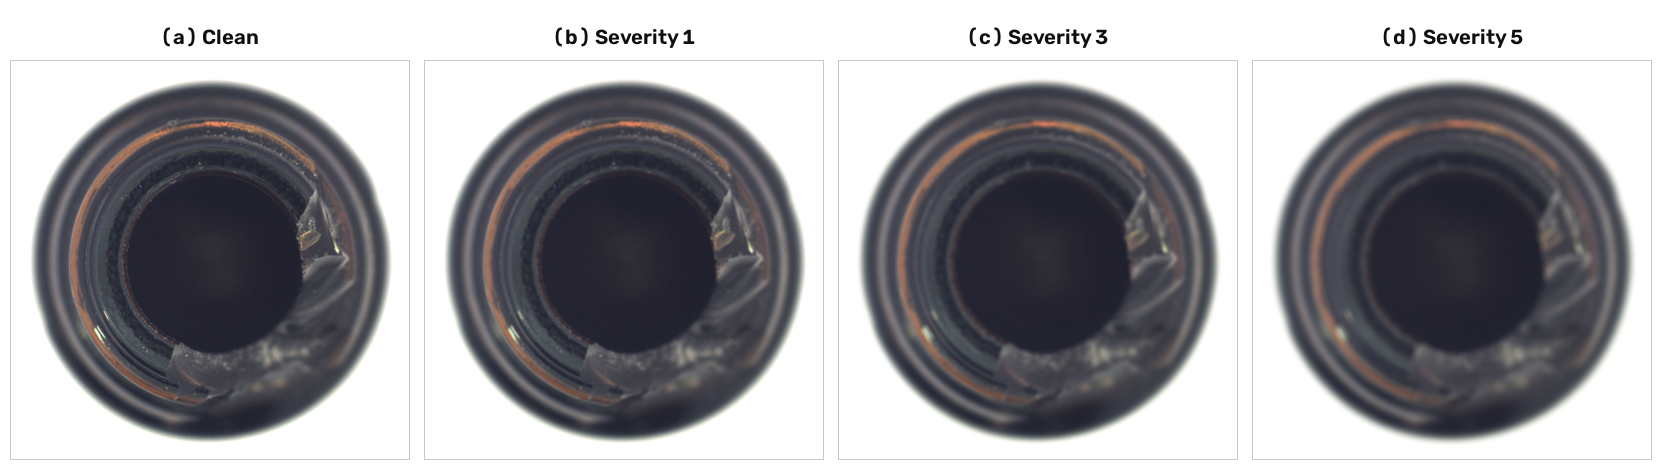
\includegraphics[width=0.96\columnwidth]{figures/fig4_bottle_defocus_progression.png}
\caption{Visual progression of optical defocus blur on a \texttt{bottle} test sample across clean input and MVTec-AD-C severity levels $1$, $3$, and $5$.}
\label{fig:defocus_progression}
\end{figure}

\begin{table}[t]
\centering
\caption{MVTec-AD-C Optical Robustness Matrix (Mask mAP@50 Across Severity Tiers 1--3 and 4--5)}
\label{tab:corruption_table}
\begin{tabular}{l c c c c}
\toprule
\multirow{2}{*}{\textbf{Corruption Type}} & \multicolumn{2}{c}{\textbf{Baseline (\texttt{EXP-08})}} & \multicolumn{2}{c}{\textbf{+2D-DWT (\texttt{EXP-10})}} \\
\cmidrule(lr){2-3} \cmidrule(lr){4-5}
 & \textbf{Sev 1--3} & \textbf{Sev 4--5} & \textbf{Sev 1--3} & \textbf{Sev 4--5} \\
\midrule
Gaussian Noise & -- & -- & -- & -- \\
Gaussian Blur  & -- & -- & -- & -- \\
Motion Blur    & -- & -- & -- & -- \\
Defocus Blur   & -- & -- & -- & -- \\
\midrule
\textbf{Mean mAP@50} & -- & -- & -- & -- \\
\textbf{Mean FAR@0.25} & -- & -- & -- & -- \\
\bottomrule
\multicolumn{5}{l}{\footnotesize `--': Reserved for completed A100 MVTec-AD-C sweeps.}
\end{tabular}
\end{table}

\subsection{Computational Efficiency}
\label{subsec:efficiency}
To verify that the single-stage polygonal segmentation backbone satisfies practical inspection throughput, we profiled inference latency on $1024 \times 1024$ frames using an NVIDIA A100-SXM4 (40 GB) GPU across PyTorch and an exported FP16 TensorRT 10.x C++ runtime. As summarized in Table~\ref{tab:edge_benchmarks}, FP16 TensorRT execution reduces neural inference latency from $32.4\text{ ms}$ ($30.8\text{ FPS}$) in PyTorch GPU to \textbf{6.7 ms} ($\approx 149.2\text{ FPS}$), a $4.8\times$ speedup well above $100\text{ FPS}$ inline sorting thresholds. Because deployment requires applying $\mathcal{T}_{\text{freq}}(I_{\text{test}})$ prior to network inference (Section~\ref{sec:methodology}), Table~\ref{tab:edge_benchmarks} explicitly reserves dedicated entries for GPU-accelerated frequency preprocessing ($\text{cuFFT}$ / $\text{DWT}$) and total end-to-end latency. End-to-end mask decoding parity across a 17-case C++ diagnostic suite confirmed $14/15$ defective categories correctly localized (e.g., Mask IoU of $0.981$ on \texttt{tile}, $0.856$ on \texttt{pill}, $0.839$ on \texttt{carpet}, $0.780$ on \texttt{grid}, and $0.668$ on \texttt{bottle}), while surfacing one missed fine thread flaw on \texttt{screw} and one nominal false positive on \texttt{hazelnut} ($0.606$).

\begin{table}[t]
\centering
\caption{Inference Latency and End-to-End Throughput on $1024 \times 1024$ Frames (NVIDIA A100-SXM4)}
\label{tab:edge_benchmarks}
\setlength{\tabcolsep}{4pt}
\begin{tabular}{l c c c l}
\toprule
\textbf{Stage / Runtime} & \textbf{Prec.} & \textbf{Latency} & \textbf{FPS} & \textbf{Viability} \\
\midrule
PyTorch CPU (Backbone) & FP32 & $184.2\text{ ms}$ & $5.4$ & Offline only \\
PyTorch GPU (Backbone) & FP16 & $32.4\text{ ms}$ & $30.8$ & Offline audit \\
\textbf{TensorRT C++ (Backbone)} & \textbf{FP16} & \textbf{6.7 ms} & \textbf{149.2} & \textbf{Inline ready} \\
\midrule
Freq. Preproc. ($\mathcal{T}_{\text{freq}}$ GPU) & FP32 & -- & -- & Pending \\
End-to-End ($\mathcal{T}_{\text{freq}}$+TRT) & FP16 & -- & -- & Pending \\
\bottomrule
\end{tabular}
\end{table}


\section{Conclusion}
\label{sec:conclusion}
In this paper, we presented an inter-domain frequency-spatial image processing framework for false-alarm-suppressed industrial surface defect segmentation under a strict defect-free training regime. On the frequency branch, we formulated an adaptive 2D-FFT periodic notch filter for repetitive texture lattices and a Haar 2D-DWT sub-band modulator for high-frequency edge enhancement, quantitatively confirming unfiltered identity roundtrip fidelity across all 2,292 unique MVTec AD RGB images ($\text{PSNR} = 52.65\text{ dB}$, $\text{SSIM} = 0.9968$ for 2D-FFT; $\text{PSNR} = 49.71\text{ dB}$, $\text{SSIM} = 0.9963$ for Haar 2D-DWT). On the spatial branch, we resolved non-power-of-two broadcast failures in multi-octave Perlin synthesis via canonical-grid bilinear mapping and integrated foreground-clamped Poisson seamless cloning with polygonal vectorization.

To address the industrial false-alarm bottleneck demonstrated in our supervised oracle evaluation ($4.50\%$--$8.78\%$ $\text{FAR@0.25}$ across 467 nominal parts), we introduced an explicit negative-sample invariant ($\rho_{\text{neg}} = 0.15$) within single-stage YOLOv11-seg optimization, while TensorRT FP16 model inference profiling confirmed real-time feasibility at $6.7\text{ ms}$ per $1024 \times 1024$ frame. Together, these components establish a unified, reproducible dual-domain evaluation and MVTec-AD-C stress-testing benchmark for defect-free industrial surface segmentation.
% TODO: Replace with final EXP-08 (Full System) & MVTec-AD-C quantitative gains once GPU sweeps finish

\textbf{Limitations:} Three technical limitations merit further investigation: (i) ultra-small, low-contrast micro-defects (such as fine thread damage on \texttt{screw}, which recorded the lowest baseline AP@50 of $0.716$) remain susceptible to detail loss under $640\times 640$ input downsampling and prototype mask strides; (ii) the selection between 2D-FFT notch filtering and 2D-DWT modulation is currently configured per material group rather than learned automatically; and (iii) local spatial synthesizers primarily model surface texture anomalies rather than global geometric or structural omissions.

\textbf{Future Work:} Future research will explore adaptive spectral periodicity gating to automate frequency-branch selection, tiled high-resolution inference for sub-millimeter micro-cracks, structural anomaly synthesis on anisotropic metallic and composite surfaces, and cross-dataset generalization across broader industrial benchmarks (e.g., VisA) under unconstrained factory-floor illumination.


\bibliographystyle{IEEEtran}
\bibliography{references}

\end{document}
